\documentclass{article}

\usepackage[T1]{fontenc}
\usepackage[polish]{babel}
\usepackage[utf8]{inputenc}
\usepackage{graphicx}
\usepackage{subcaption} 
\usepackage[margin=2cm]{geometry}

\title{Raport Zadanie NUM1}
\date{14.10.2023}
\author{Tomasz Dziób}

\begin{document}
  \maketitle
  \newpage
  \section{Wstęp}
  Poniższy raport dotyczy zadania numerycznego NUM1 z listy 1.
Załączony program o nazwie \textit{num1.cpp} został napisany w języku \textit{C++}, do wykonania
  wykresów został użyty \textit{GnuPlot}. Do obsługi GnuPlota w cpp został 
  wykorzystany plik nagłówkowy \textit{gnuplot-iostream.h}.
    \subsection{Jak uruchomić program?}
    Razem z załączonymi plikami znajdziemy Makefile który służy do
    uruchomienia programu komendą: \textit{make run}.
  \section{Spodziewany wynik}
   Oczekujemy, że błąd przybliżenia będzie maleć w miarę zmniejszania wartości
   h i zbliżania się do zera. Jednakże, dla bardzo małych wartości h, może 
   pojawić się błąd zaokrągleń i utrata dokładności.

  \section{Użyta metoda}
  Wyniki uzyskujemy poprzez przybliżenie pochodnej funkcji tzn.
  wartość bezwzględną z różnicy wartości pochodnej i
  aktualnie używanego wzoru.

  \section{Uzyskany wynik}
  Spoglądając na wykresy jesteśmy wstanie zauważyć kilka różnic. Pozwoliłem sobie
  stworzyć dwa wykresy jeden dla podpunktu a), drugi dla podpunktu b), porównujące
  typy \textit{float} oraz \textit{double}.

  \begin{figure}[!ht]
      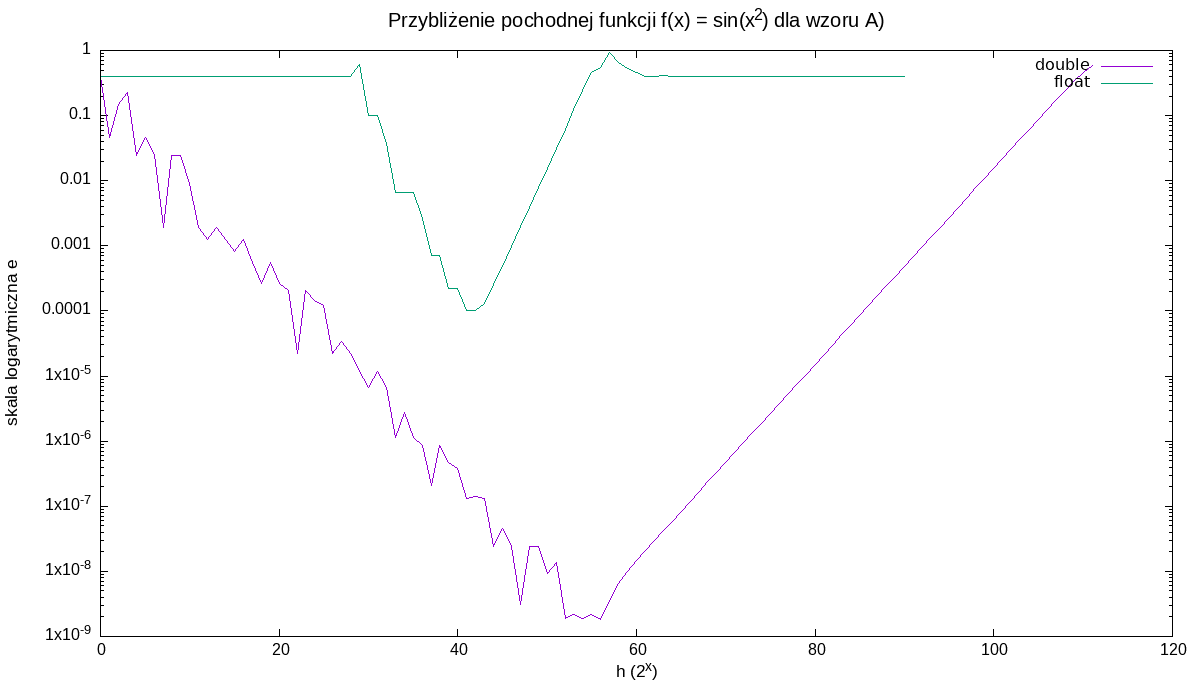
\includegraphics[width=\linewidth]{wyniki_A.png}
      \caption{Porównanie typów zmiennoprzecinkowych dla podpunktu a)}
    \end{figure}

    Dla pierwszej funkcji jesteśmy wstanie wyraźnie wyróżnić trzy różne zachowania
    funkcji. Pierwszą z nich oczekiwany błąd w postaci szumu na wykresie, jest on 
    zdecydowanie prostszy do zauważenia dla typu double. W okolicy punktu granicy błędu
    występuje ustabilizowanie wartości jednak szum dalej wystepuje w nieznacznej ilości.
    Po przekroczeniu wspomnianego wcześniej punktu wykres przyjmuje wręcz linearny przyrost. 


    Spoglądając na drugi wykres widać inne zachowanie. Po spodziewanym szumie za punktem 
    granicy błędu, funkcja odrazu zaczyna przyrost liniowy. W porównaniu do pierwszej 
    funkcji widać wiekszą dokładość sięgającą praktycznie do $1 \cdot 10^{-12}$, podczas
    gdy dla podpunktu a) wartości double ledwo sięgają wartości $1 \cdot 10^{-9}$.

  \begin{figure}[!ht]
    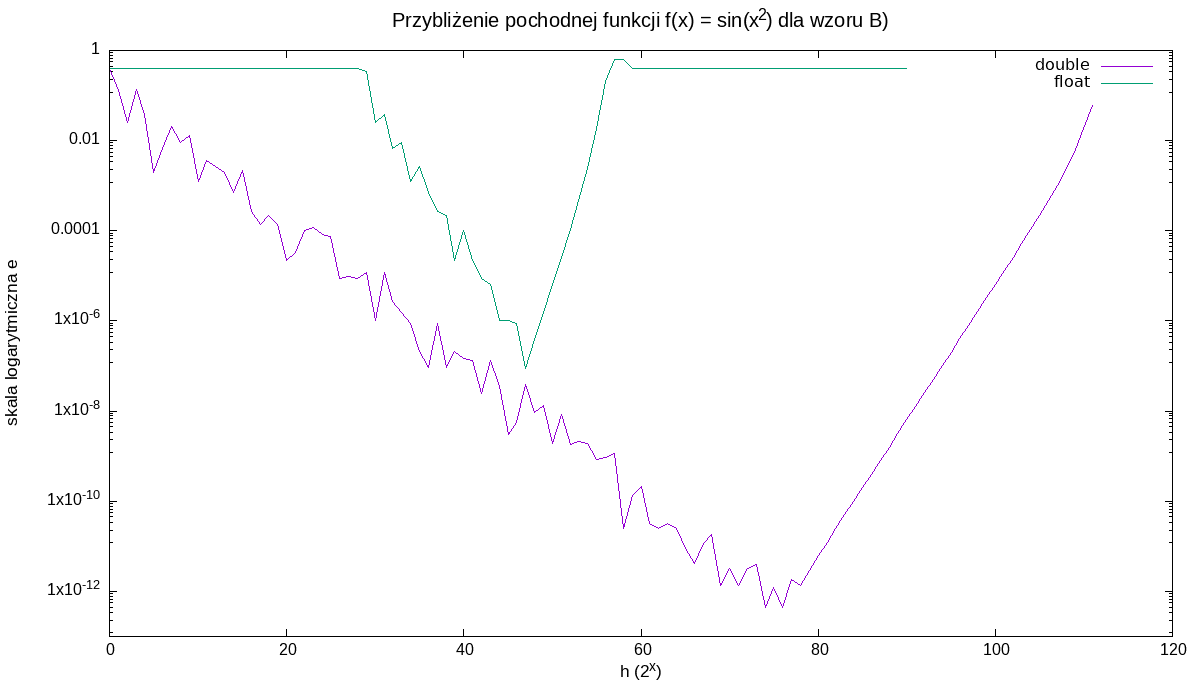
\includegraphics[width=\linewidth]{wyniki_B.png}
    \caption{dla danych typu double}
  \end{figure}
   
  Obserwowana zależność błędu przybliżenia od wartości h jest zgodna z oczekiwaniami 
  teoretycznymi. Błąd maleje w miarę zmniejszania wartości h i zbliżania się do zera.
  Dla bardzo małych wartości h, błąd zaczyna rosnąć ze względu na błędy zaokrągleń
   w arytmetyce zmiennoprzecinkowej.
  
  Ogólne wnioski, które można sformułować mówią, że typu float jest o wiele gorszy
  jeśli chodzi o dokładność, jest to wynikową mniejszego zakresu.
  Wzór B zapewnia mniejszy błąd w porównaniu do wzoru A dla tych samych wartości h.
  jest bardziej stabilny i dokładny, co jest widoczne. Wykresy na skali 
  logarytmicznej pozwalają lepiej zrozumieć zachowanie błędu przybliżenia.

\end{document}
